%%%%%%%%%%%%%%%%%%%%%%%%%%%%%%%%%%%%%%%%%%%%%%%%%%%%%%%%%%%%%%%%%%%%%%
% LaTeX Example: Project Report
%
% Source: http://www.howtotex.com
%
% Feel free to distribute this example, but please keep the referral
% to howtotex.com
% Date: March 2011 
% 
%%%%%%%%%%%%%%%%%%%%%%%%%%%%%%%%%%%%%%%%%%%%%%%%%%%%%%%%%%%%%%%%%%%%%%
% How to use writeLaTeX: 
%
% You edit the source code here on the left, and the preview on the
% right shows you the result within a few seconds.
%
% Bookmark this page and share the URL with your co-authors. They can
% edit at the same time!
%
% You can upload figures, bibliographies, custom classes and
% styles using the files menu.
%
% If you're new to LaTeX, the wikibook is a great place to start:
% http://en.wikibooks.org/wiki/LaTeX
%
%%%%%%%%%%%%%%%%%%%%%%%%%%%%%%%%%%%%%%%%%%%%%%%%%%%%%%%%%%%%%%%%%%%%%%
% Edit the title below to update the display in My Documents
%\title{Project Report}
%
%%% Preamble
\documentclass[paper=a4, fontsize=11pt]{scrartcl}
\usepackage[utf8x]{inputenc}

\usepackage{fourier}

\usepackage[portuguese]{babel}															% English language/hyphenation
\usepackage[protrusion=true,expansion=true]{microtype}	
\usepackage{amsmath,amsfonts,amsthm} % Math packages
\usepackage[pdftex]{graphicx}	
\usepackage{url}
\usepackage{multirow}
\usepackage{hyperref}
\usepackage{listings}
\usepackage{xcolor}
\usepackage{graphicx}
\usepackage{float}

%%% Custom sectioning
\usepackage{sectsty}
\allsectionsfont{\centering \normalfont\scshape}


%%% Custom headers/footers (fancyhdr package)
\usepackage{fancyhdr}
\pagestyle{fancyplain}
\fancyhead{}											% No page header
\fancyfoot[L]{}											% Empty 
\fancyfoot[C]{}											% Empty
\fancyfoot[R]{\thepage}									% Pagenumbering
\renewcommand{\headrulewidth}{0pt}			% Remove header underlines
\renewcommand{\footrulewidth}{0pt}				% Remove footer underlines
\setlength{\headheight}{13.6pt}


%%% Equation and float numbering
\numberwithin{equation}{section}		% Equationnumbering: section.eq#
\numberwithin{figure}{section}			% Figurenumbering: section.fig#
\numberwithin{table}{section}				% Tablenumbering: section.tab#


\lstset{ %
	backgroundcolor=\color{white},   % choose the background color; you must add \usepackage{color} or \usepackage{xcolor}
	basicstyle=\footnotesize,        % the size of the fonts that are used for the code
	breakatwhitespace=false,         % sets if automatic breaks should only happen at whitespace
	breaklines=true,                 % sets automatic line breaking
	captionpos=b,                    % sets the caption-position to bottom
	commentstyle=\color{red},    % comment style
	extendedchars=true,              % lets you use non-ASCII characters; for 8-bits encodings only, does not work with UTF-8
	frame=single,                    % adds a frame around the code
	keepspaces=true,                 % keeps spaces in text, useful for keeping indentation of code (possibly needs columns=flexible)
	keywordstyle=\color{blue},       % keyword style
	language=C,                 % the language of the code
	otherkeywords={func, :=, ++, sync, ==},            % if you want to add more keywords to the set
	numbers=left,                    % where to put the line-numbers; possible values are (none, left, right)
	numbersep=10pt,                   % how far the line-numbers are from the code
	numberstyle=\tiny\color{gray}, % the style that is used for the line-numbers
	%rulecolor=\color{black},         % if not set, the frame-color may be changed on line-breaks within not-black text (e.g. comments (green here))
	showspaces=false,                % show spaces everywhere adding particular underscores; it overrides 'showstringspaces'
	showstringspaces=false,          % underline spaces within strings only
	showtabs=false,                  % show tabs within strings adding particular underscores
	tabsize=2,                       % sets default tabsize to 2 spaces
}

%%% Maketitle metadata
\newcommand{\horrule}[1]{\rule{\linewidth}{#1}} 	% Horizontal rule

\title{
		%\vspace{-1in} 	
		\usefont{OT1}{bch}{b}{n}
		\normalfont \normalsize \textsc{Instituto de Matemática e Estatística\\Universidade de São Paulo} \\ [25pt]
		\horrule{0.5pt} \\[0.4cm]
		\huge EP2 - MAC0438 \\
		\horrule{2pt} \\[0.5cm]
}
\author{
		\normalfont 								\normalsize
        João Marco Maciel da Silva 7577598\\
        \normalsize
        \today
}
\date{}


%%% Begin document
\begin{document}
\maketitle
\section{Configuração da Máquina}
Informações extraídas por \textit{dmidecode}, \textit{uname} e \textit{lsb\_release}.\\

\begin{tabular}{lll}
	\multirow{3}{*}{Baseboard} & Type& Laptop\\
	& Manufacturer& SAMSUNG ELECTRONICS CO., LTD.\\
	& Product Name& R480/R431/R481\\
	\hline
	\multirow{5}{*}{Processor}& Family& Core i3\\
	& Max Speed& 3200MHz\\
	& Core Count& 2\\
	& Thread Count& 4\\
	& Characteristics& 64-bit capable\\
	\hline
	\multirow{5}{*}{Memory}& Type& DDR3\\
	& Data Width& 64 bits\\
	& Speed& 667MHz\\
	& Number of Devices& 2\\
	& Size& 2048MB x2\\
	\hline
	\multirow{3}{*}{Cache Size}& L1& 32 kB\\
	& L2& 256 kB\\
	& L3& 3072 kB\\
	\hline
	\multirow{3}{*}{uname}& OS& Linux\\
	& Kernel Release& 3.19.5-100.fc20.x86\_64\\
	& Processor type& x86\_64\\
	\hline
	\multirow{1}{*}{lsb\_release}& Description& Fedora 20\\
\end{tabular}

Os testes foram todos feitos em um terminal sem interface gráfica
\section{Testes}
\subsection{Medição dos tempos}
Os tempos foram medidos com o \textit{script} que acompanha o EP.\\
A variável \textit{TIMEFORMAT} foi configurada para que o comando \textit{time} retornasse os dados de tempo em um formato fácil de manipular.\\
Do comando \textit{time} foi retornado o tempo de usuário, tempo de sistema, tempo real e percentual de CPU usado.\\

\subsection{Parâmetros e repetições}
Para cada entrada foram executadas 30 repetições.\\
Esse tamanho de amostra é um bom tamanho mínimo para que as médias das amostras possam ser aproximadas por uma normal satisfatoriamente.

\subsubsection{1º parâmetro - número de processos}
O EP foi testado nessa máquina com até 150 processos, porém o tempo execução para mais que 15 processos é muito alto e não possível retirar medidas estatísticas em tempo viável.\\
Para as medidas que estão nos gráficos foram feitos testes com até 10 processos.\\

\subsubsection{2º parâmetro - \textit{f} ou \textit{m}}
Para cada conjunto de testes foram feitos testes com \textit{f} e com \textit{m}.\\

\subsubsection{3º parâmetro - precisão}
Foram feitos testes com precisão de $10^{-10}$, $10^{-100}$, $10^{-1000}$, $10^{-10000}$ e $10^{-10000}$, tanto para \textit{f} quanto para \textit{m}.\\

\subsubsection{4º parâmetro - valor de \textit{x}}
Foram usados quatro valores de \textit{x}, $x=1$, $x=3,14159265359$, $x=0.1$ e $x=0$.\\

\subsubsection{5º parâmetro - s, d ou nada}
Todos os testes sem o 5º argumento também foram executados com o argumento \textit{d} e quando não variando no 1º argumento também com o argumento \textit{s}.\\

\subsection{Geração dos gráficos}
Os gráficos e cálculos estatísticos foram feitos com ajuda do Google Spreadsheets e os dados originais podem ser encontrados \href{https://docs.google.com/spreadsheets/d/10F9Elp18penPIfwJ-gPzf1omaWTKKJAMlrtgMT_AK0c/edit?usp=sharing}{aqui}.\\

\subsection{Resultados}

\begin{figure}[H]
	\centering
	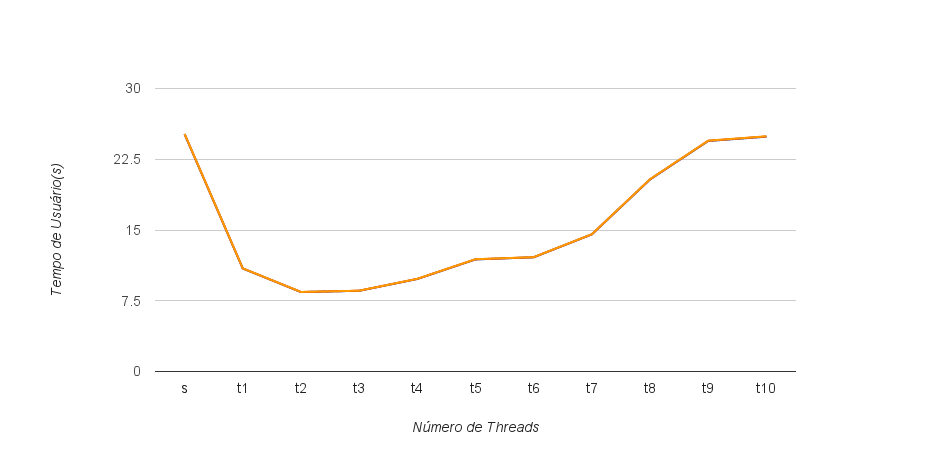
\includegraphics[width=0.9\textwidth]{image}
	\caption{Média do tempo para x = 3.141592654, f = 1000}
	\label{image1}
\end{figure}

\begin{figure}[H]
	\centering
	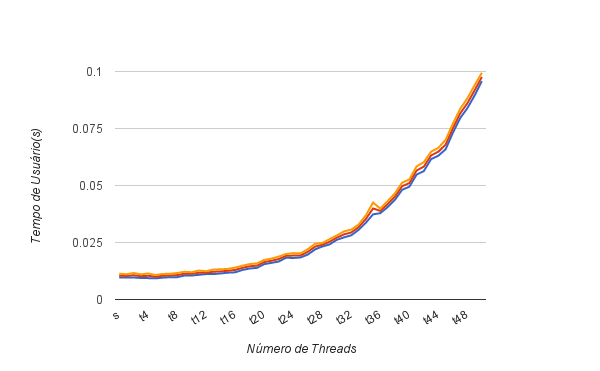
\includegraphics[width=0.8\textwidth]{image2}
	\caption{Média do tempo para x = 0, f = 100000}
	\label{image2}
\end{figure}

\begin{figure}[H]
	\centering
	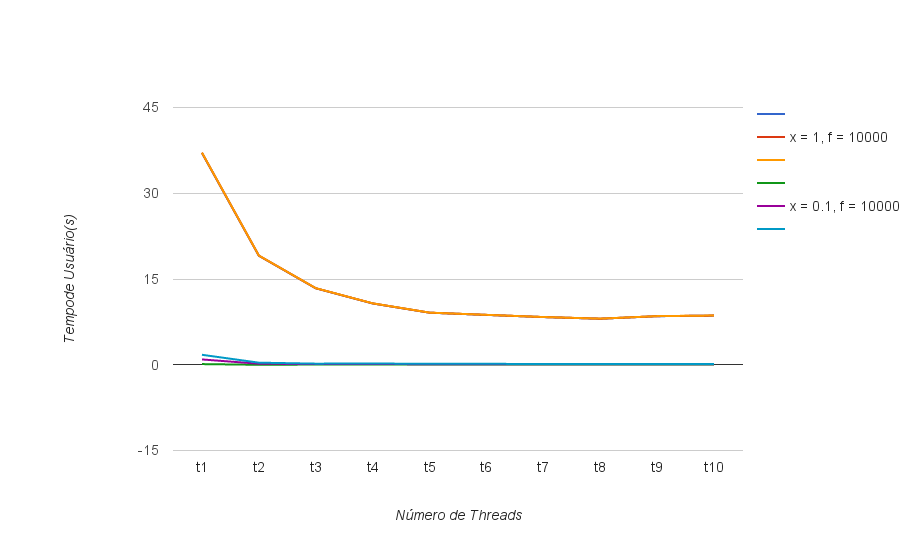
\includegraphics[width=\textwidth]{image3}
	\caption{Médias do tempo para x = 1 e x = 0.1, f = 10000}
	\label{image3}
\end{figure}

\begin{figure}[H]
	\centering
	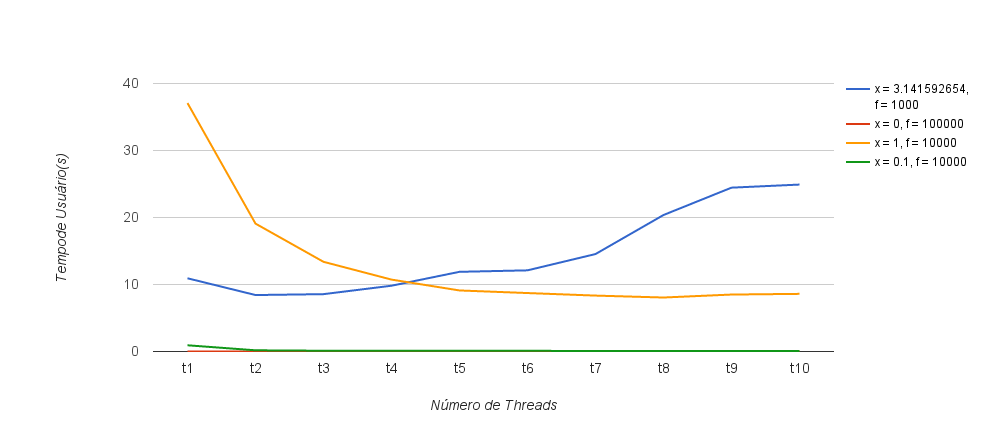
\includegraphics[width=\textwidth]{image4}
	\caption{Compração entre as médias}
	\label{image4}
\end{figure}

O gráfico \ref{image1} mostra o formato esperado do gráfico do número de processos pelo tempo. É esperado esse formato pois o tempo diminui até uma certa quantidade de processos e depois há um \textit{overhead} para gerenciar os processos e há um excesso de cálculos, que por si só são custosos. É esperado que o tempo de \textit{s} seja muito maior que \textit{t1} e \textit{t2}, pois não há nenhuma concorrência nesse caso.\\

O gráfico \ref{image2} mostra o formato esperado do gráfico do número de processos pelo tempo. Como $x = 0$ os termos são todos iguais a 0, logo ela acaba sempre depois da primeira rodada. Então espera-se que o gráfico seja sempre crescente. As linhas coloridas ao redor mostram o intervalo de confiança para uma confiança de 99\%, no gráfico \ref{image1} essas linhas se fundem e não é possível verificá-las.\\

O gráfico \ref{image3} mostra as curvas de dois valores, um decimal e outro inteiro. A diferença entre os dois é, possivelmente, por conta do decimal ser menor e precisar de menos turnos para chegar ao valor da precisão. No caso de 10 processos e $f=10000$, $x=1$ precisou de 18 rodadas e $x=0.1$ precisou de 14. É possível verificar que o formato da curva é o mesmo, mas que a área dos dois é completamente diferente. \\

A última conclusão que pode ser retirada com os resultados é que a curva para um \textit{x} decimal com mais casas decimais deve inverter a derivada da cruva antes de um \textit{x} com menos casas decimais. Esta conclusão pode ser percebida no gráfico \ref{image4}, onde a curva com $x=3.141592654$ inverte já com q igual a 4, enquanto os outros com $q>10$.\\

\section{Barreiras utilizadas}
Foram utilizadas duas barreiras diferentes.
A primeira, criada por mim, usa-se de uma exclusão mútua e um contador. Removendo o que é específico da aplicação seria:
\begin{lstlisting}
type Barreira func()
func newBarreira(q int) Barreira {
	mutex := &sync.Mutex{}
	cond  := sync.NewCond(mutex)
	count := 0
	
	return func() {
		mutex.Lock()
		count++
		if count == q+1 {
			count = 0
			cond.Broadcast()
		} else {
			cond.Wait()
		}
		mutex.Unlock()
	}
}
\end{lstlisting}
Primeiro ele inicializa a barreira com tamanho q+1 (o +1 é para incluir o caminho padrão) e cada processo que chega na barreira chama a função da barreira. Dentro da função ele entra em uma área de exclusão mútua, incrementa o contador e se foro último lança uma mensagem broadcast para todos que estiverem esperando, caso contrário apenas espera. No final libera a trava.\\
Esse código na sintaxe utilizada na aula é aproximadamente equivalente a:
\begin{lstlisting}
sem mutex = 1
int count = 0
boolean cond = false

barreira {
	P(mutex)
	count++
	if (count == q+1) {
		count = 0
		cond = true
	} else {
		< V(mutex); await(cond) >
		P(mutex)
	}
	V(mutex)
}
\end{lstlisting}

A outra barreira, um pouco mais discreta usa-se de uma estrutura própria da linguagem.
\begin{lstlisting}
// Inicializacao
	sumPart = make(chan *big.Rat)
	
// Em cada processo de calculo do cosseno:
	sumPart <- sum
// significa insere o conteudo de "sum" no buffer de tamanho variavel sumPart.

// No processo original:
	for i := 0; i < q; i++ {
		cos.Add(cos, <-sumPart)
	}
// Significa para i=0 a q
		< await(buffer!=vazio);
		sum recebe proximo elemento do buffer >
		executa cos.Add(cos, sum)
\end{lstlisting}
Essa estrutura é chamada na linguagem de \textit{canal}.\\
O trecho que está no processo original funciona como uma berreira, fazendo o processo esperar até que haja alguma mensagem no canal.

\section{Biblioteca de alta precisão}
Foi utilizado a biblioteca padrão da linguagem para número com alta precisão.

\subsection{Naturais}
Números naturais nessa biblioteca são representados como um vetor de tamanho variável de inteiros de 64bit sem sinal, onde 0's precedentes são eliminados a cada operação feita e, assim sendo, o vetor vazio ou nulo representam o 0.\\

\subsection{Inteiros}
Inteiros são structs compostas por um natural e um booleano representando o sinal.\\

\subsection{Racionais}
Racionais são structs contendo um inteiro denominador \textit{b} e um inteiro numerador \textit{a}, sendo assim um racional na forma ${a}\over{b}$. Sendo considerado o sinal apenas de a para determinar o sinal do racional. Sendo assim a precisão do número é tão grande quanto se desejar.\\

\subsection{Vantagem}
A grande vantagem do uso desta biblioteca é que é possível obter \textbf{qualquer} precisão, \textbf{não} apenas limitado aos \textbf{100k} exigidos pelo execício.\\

\subsection{Desvantagem}
A grande desvantagem do uso desta biblioteca é que não há controle algum sobre a precisão, o que torna as operações pesadas  demais em pouquissimas rodadas do algorítmo, ou seja, ela é (muito) \textbf{lento}.\\


%%% End document
\end{document}